\documentclass{standalone}
\usepackage[utf8]{inputenc}
\usepackage{tikz}
\usepackage{color}
\usetikzlibrary{arrows,shapes,positioning,shadows,trees}

\tikzset{
  basic/.style  = {draw, text width=3cm, drop shadow, font=\sffamily, rectangle},
  root/.style   = {basic, rounded corners=2pt, thin, align=center,
                   fill=yellow!60},
  level 2/.style = {basic, rounded corners=6pt, thin,align=center, fill=yellow!40,
                   text width=15em},
  level 3/.style = {basic, thin, align=left, fill=yellow!20, text width=8em}
}

\begin{document}

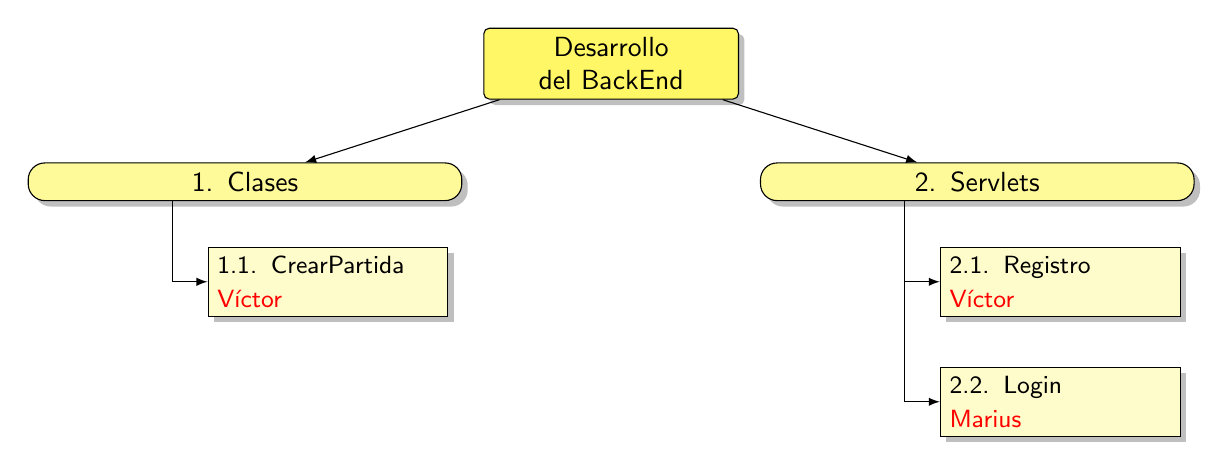
\begin{tikzpicture}[
  level 1/.style={sibling distance=93mm},
  edge from parent/.style={->,draw},
  >=latex]

% raiz inicial
\node[root] {Desarrollo del BackEnd}
% The first level, as children of the initial tree
  child {node[level 2] (c1) {1. Clases}}
  child {node[level 2] (c2) {2. Servlets}};

% The second level, relatively positioned nodes
\begin{scope}[every node/.style={level 3}]
\node [below of = c1,node distance=0.5in, xshift=30pt] (c11) {\small{1.1. CrearPartida} \\ \textcolor{red}{\small{Víctor}}};

\node [below of = c2, xshift=30pt, node distance = 0.5in] (c21) {\small{2.1. Registro}\\ \textcolor{red}{\small{Víctor}}};
\node [below of = c21, node distance=0.6in] (c22) {\small{2.2. Login}\\ \textcolor{red}{\small{Marius}}};
\end{scope}

\foreach \value in {1}
  \draw[->] (c1.195) |- (c1\value.west);
\foreach \value in {1,...,2}
  \draw[->] (c2.195) |- (c2\value.west);
\end{tikzpicture}

\end{document}
